%! TeX root = ../../main-en.tex
% 译自: chapters/zh/ch04.tex @ a1b3a4b:chapters/zh/ch04.tex
\chapter{Memory and Pointers}
\label{chap:memory}

When Chapter~\ref{chap:c-basics} talked about \texttt{scanf}, it left a little mystery: when we read a value into a variable, why do we put an \texttt{\&} in front of the variable's name? To answer that, we first have to find out something else: where do the variables of a program actually live?

The first half of this chapter is about memory: what a program looks like in memory, where its data lives, what the stack is, what the heap is, and why user programs are not allowed to touch the operating system kernel. These are basic ideas of computer architecture. Someone just starting C may not need them right away, but once you have this picture in your head, pointers, operating systems and CPUs all become much easier to learn. The second half is about pointers---variables that hold addresses. With the picture from the first half, pointers are not mysterious at all.

The examples for this chapter are in the \texttt{code/en/ch04/} directory. Run \texttt{make} to build them and \texttt{make test} to check them. To keep the addresses short and easy to read, most of the programs are built as \emph{32-bit} programs. What ``32-bit'' and ``64-bit'' mean is explained in Section~\ref{sec:bits}.

To build a 32-bit program, just add \texttt{-m32} to \texttt{gcc} (you need to install \texttt{gcc-multilib} first):
\begin{minted}[linenos=false]{text}
gcc -m32 addr.c -o addr
./addr
\end{minted}
Our computer actually runs 64-bit Linux. To make the addresses in the book exactly the same as on real 32-bit Linux, and the same every time, this chapter's Makefile and scripts add a few more options when they build and run the programs (they are explained in the comments of \texttt{code/en/ch04/Makefile}; you can ignore them). So when you run the programs yourself, you will most likely see different addresses from the book. That is perfectly normal.

\section{Memory: A Row of Numbered Houses}
\label{sec:mem-street}

Think of memory as a very, very long street lined with identical little houses. Each house has room for just one \emph{byte}\lazynote{Byte}{8 binary digits (bits), enough for a number from 0 to 255. Memory gets one house number per byte.}: 8 binary digits, enough to hold one number between 0 and 255. Every house has a house number, and that number is its \emph{address}. To read or write memory, the CPU has to give the house number: ``Bring me whatever is in house number \texttt{0xbffffdf4}.''

In C, put \texttt{\&} in front of a variable's name and you get the variable's address:

\codefile{code/en/ch04/addr.c}{Where do the variables live?}{lst:addr}

\inputminted[linenos=false]{text}{code/en/ch04/out/addr.txt}

A few notes:
\begin{itemize}
  \item \texttt{\&a} reads as ``the address of a''. \texttt{printf} prints addresses with \texttt{\%p}. The \texttt{(void *)} in front tells \texttt{printf} ``this is an address''. Just copy it as it is.
  \item \texttt{sizeof(int)} works out how many bytes an \texttt{int} takes; print it with \texttt{\%zu}. On our computer an \texttt{int} takes 4 bytes, so it needs 4 houses.
  \item Addresses are written in \emph{hexadecimal}\lazynote{Hexadecimal}{Counting in sixteens, using \texttt{0}--\texttt{9} and \texttt{a}--\texttt{f}. Two hex digits make exactly one byte.}, and the \texttt{0x} in front marks a hexadecimal number. Hexadecimal counts in sixteens, using the 16 symbols \texttt{0}--\texttt{9} and \texttt{a}--\texttt{f}: \texttt{a} is 10, \texttt{f} is 15 and \texttt{0x10} is 16. Addresses are big numbers and would be too long in decimal. Hexadecimal is just right: two hex digits make exactly one byte.
\end{itemize}

\texttt{a} lives at \texttt{0xbffffdf4} and \texttt{b} lives at \texttt{0xbffffdf8}, exactly 4 apart: \texttt{a} takes up the 4 houses from \texttt{0xbffffdf4} to \texttt{0xbffffdf7}, and \texttt{b} lives right next door (Figure~\ref{fig:houses}).

\begin{figure}[htbp]
  \begin{lazywide}
  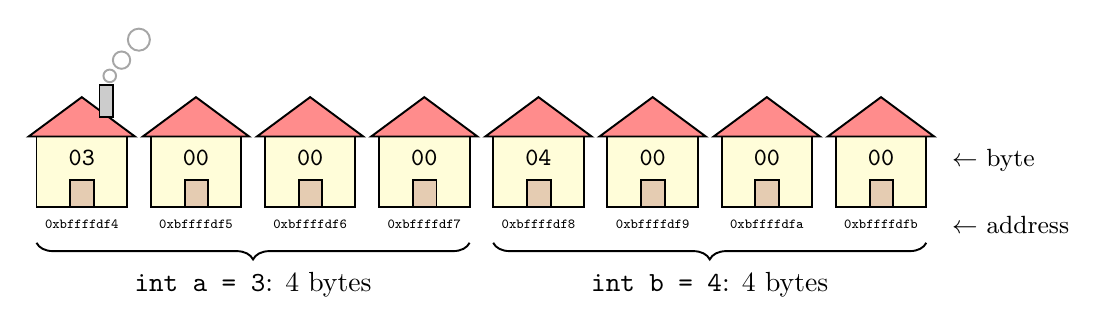
\begin{tikzpicture}[line width=0.7pt]
    \foreach \i/\v/\n in {0/03/f4, 1/00/f5, 2/00/f6, 3/00/f7, 4/04/f8, 5/00/f9, 6/00/fa, 7/00/fb} {
      \pgfmathsetmacro\x{\i*1.45}
      \filldraw[fill=yellow!15] (\x,0) rectangle +(1.15,0.9);
      \filldraw[fill=red!45] (\x-0.1,0.9) -- +(0.675,0.5) -- +(1.35,0) -- cycle;
      \filldraw[fill=brown!40] (\x+0.43,0) rectangle +(0.3,0.35);
      \node[font=\ttfamily\small] at (\x+0.575,0.63) {\v};
      \node[font=\ttfamily\tiny] at (\x+0.575,-0.22) {0xbffffd\n};
    }
    % Chimney and smoke
    \filldraw[fill=gray!40] (0.8,1.15) rectangle (0.97,1.55);
    \foreach \r/\dx/\dy in {0.08/0.05/0.12, 0.11/0.2/0.32, 0.14/0.42/0.58}
      \draw[gray!70] (0.88+\dx,1.55+\dy) circle (\r);
    \draw[decorate, decoration={brace, mirror, amplitude=6pt}]
      (0,-0.45) -- (5.5,-0.45) node[midway, below=7pt] {\texttt{int a = 3}: 4 bytes};
    \draw[decorate, decoration={brace, mirror, amplitude=6pt}]
      (5.8,-0.45) -- (11.3,-0.45) node[midway, below=7pt] {\texttt{int b = 4}: 4 bytes};
    \node[font=\small, anchor=west] at (11.5,0.6) {$\leftarrow$ byte};
    \node[font=\small, anchor=west] at (11.5,-0.22) {$\leftarrow$ address};
  \end{tikzpicture}
  \caption{Memory is a row of numbered houses, one byte per house}
  \label{fig:houses}
  \end{lazywide}
\end{figure}

Look closely at the figure. How does the number 3 fit into 4 bytes? It is stored as \texttt{03 00 00 00}: the lowest byte of the number goes into the house with the smallest address. This way of storing numbers is called \emph{little-endian}\lazynote{Little-endian}{The lowest byte of a number goes at the smallest address. The opposite is big-endian.}. Both x86 and RISC-V processors store numbers this way.

\section{How Long Is an Address? 16, 32 and 64 Bits}
\label{sec:bits}

How long a house number can be decides how many houses the street can have. If an address has $n$ binary digits, there are $2^n$ different house numbers, so the CPU can reach $2^n$ bytes of memory. When people say ``32-bit'' or ``64-bit'', this is what they mean here: how many bits an address has.

The same program can be built as a 32-bit program or as a 64-bit one:

\codefile{code/en/ch04/bits.c}{How big is an address?}{lst:bits}

\inputminted[linenos=false]{text}{code/en/ch04/out/bits.txt}

In a 32-bit program an address takes 4 bytes, which is 8 digits in hexadecimal. In a 64-bit program it takes 8 bytes, and the printed address is a lot longer. This chapter uses 32-bit addresses in its examples simply because they are short and easy to read. The ideas are exactly the same for 32 and 64 bits.

\begin{figure}[htbp]
  \begin{lazywide}
  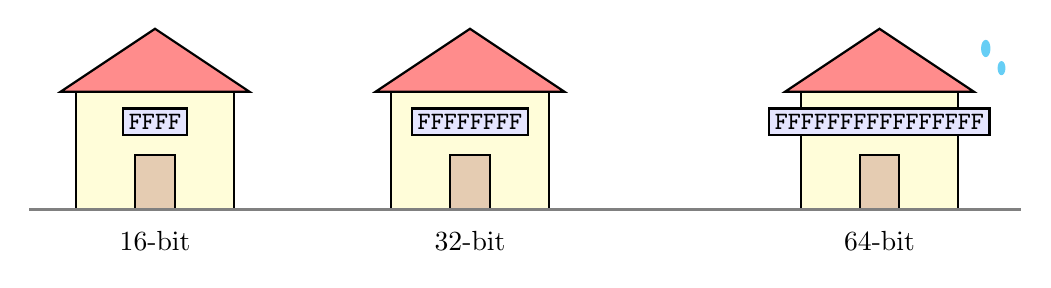
\begin{tikzpicture}[line width=0.8pt]
    \foreach \x/\plate/\label in {0/FFFF/16-bit, 4.0/FFFFFFFF/32-bit, 9.2/FFFFFFFFFFFFFFFF/64-bit} {
      \filldraw[fill=yellow!15] (\x,0) rectangle +(2.0,1.5);
      \filldraw[fill=red!45] (\x-0.2,1.5) -- +(1.2,0.8) -- +(2.4,0) -- cycle;
      \filldraw[fill=brown!40] (\x+0.75,0) rectangle +(0.5,0.7);
      \node[draw, fill=blue!10, font=\ttfamily\small, inner sep=2pt] at (\x+1.0,1.12) {\plate};
      \node at (\x+1.0,-0.4) {\label};
    }
    % The 64-bit house number is too long to fit, and the house is sweating
    \fill[cyan!60] (11.55,2.05) ellipse (0.06 and 0.11);
    \fill[cyan!60] (11.75,1.8) ellipse (0.05 and 0.09);
    \draw[gray, line width=1pt] (-0.6,0) -- (12.0,0);
  \end{tikzpicture}
  \caption{House numbers keep getting longer}
  \label{fig:plates-grow}
  \end{lazywide}
\end{figure}

Why did addresses grow from 16 bits to 32 bits, and then to 64 bits? In short: memory kept getting bigger, and we ran out of house numbers (Table~\ref{tab:bits}).

\begin{table}[htbp]
  \begin{lazywide}
  \small
  \caption{Address bits and the memory they can reach}
  \label{tab:bits}
  \begin{tabular}{L{3.8cm}L{2.4cm}L{5.4cm}L{1.8cm}}
    \toprule
    Address bits & Memory it can reach & Typical processors & When \\
    \midrule
    16 bits & 64\,KB & Intel 8080, MOS 6502 (Apple II, NES) & 1970s \\
    20 bits (pieced together with segments) & 1\,MB & Intel 8086 (IBM PC) & 1978 \\
    32 bits & 4\,GB & Intel 80386 & 1985 \\
    64 bits (48 actually used today) & 256\,TB & AMD64 (AMD Opteron) & 2003 \\
    \bottomrule
  \end{tabular}
  \end{lazywide}
\end{table}

\paragraph{16 bits: a little street of 64 KB.}
Early microprocessors, such as the Intel 8080 and the MOS 6502 (used in Apple's Apple II computer and in Nintendo's NES game console), had 16-bit addresses. $2^{16} = 65\,536$, so they could reach at most 64\,KB of memory. In the 1970s that was a lot, but programs kept getting bigger, and soon it was not enough.

In 1978 Intel brought out the 8086. Inside it was still 16-bit, but it found a trick to reach 1\,MB of memory with 20-bit addresses: memory was divided into pieces called segments, and an address was made of two parts, a ``segment'' and an ``offset inside the segment''. The real address was ``segment\,${}\times 16 +{}$\,offset''. This is called \emph{segmentation}\lazynote{Segmentation}{The 8086's trick: address = segment $\times$ 16 + offset, two 16-bit numbers that together make a 20-bit address.}. Segmentation worked, but it was awkward: one address needed two numbers, the same place could be written in many different ways, and C programmers even had to tell ``near pointers'' from ``far pointers''. The IBM PC used processors from the 8086 family. Part of the 1\,MB was kept for the display and the BIOS, which left only 640\,KB for programs. ``640\,KB of memory'' is something many programmers of that time still remember.

\paragraph{32 bits: a flat 4 GB avenue.}
In 1985 Intel brought out the 80386. Addresses became 32 bits long, and $2^{32}$ bytes is 4\,GB. Even more important, segments were no longer needed: all the addresses from \texttt{0x00000000} to \texttt{0xffffffff} lined up along one long, straight street. This is called a \emph{flat} address space. The 80386 also supported \emph{paging}\lazynote{Paging}{Cutting memory into pages (usually 4\,KB each); every page can be mapped and protected on its own.} in hardware, which lets the operating system give every program its own complete 4\,GB virtual address space (more on this at the end of Section~\ref{sec:layout}). In 1991, a Finnish university student called Linus Torvalds started writing Linux on his own 80386 computer. Linux 0.11, mentioned in the preface, was written for the 80386 too.

\paragraph{64 bits: even 4 GB is not enough.}
Back then 4\,GB looked far too big to ever fill up. Yet in less than twenty years, ordinary computers came with 4\,GB of memory. What's more, a 32-bit program cannot even use all 4\,GB of addresses: 32-bit Linux keeps 1\,GB of them for the operating system kernel (Section~\ref{sec:kernel-space}), and 32-bit Windows gives programs only 2\,GB by default. Databases, video editors and big games were all squashed under this low ceiling. In 2003 AMD brought out AMD64, a 64-bit x86 processor, and Intel soon followed. Today almost every computer and phone is 64-bit.

$2^{64}$ bytes is 16\,EB (about 17 billion GB), far more than any computer needs today. So today's x86-64 processors actually use only 48-bit addresses, which can reach 256\,TB; newer processors can use 57 bits. The address \texttt{0x7fffffffecdc} printed by \texttt{bits64} above has 12 hex digits---exactly 48 bits.

\paragraph{32 bits is not out of date.}
A 64-bit processor can also run 32-bit programs. That is why we can build 32-bit programs with \texttt{gcc -m32} and run them on 64-bit Linux. The \texttt{0xbffffdf4} printed by \texttt{bits32} above is a typical stack address in a 32-bit Linux program. The little chips inside washing machines, routers and fitness bands are still mostly 32-bit, and RISC-V comes in both 32-bit (RV32) and 64-bit (RV64) versions. Shorter addresses mean a simpler chip. If you are building a CPU from scratch, 32 bits is a fine place to start.

\section{Where a Program Lives in Memory}
\label{sec:layout}

When a program runs, its code, its global variables and its local variables all need somewhere to live in memory. Where do they live? Let us write a program and see:

\codefile{code/en/ch04/layout.c}{Where do the parts of a program live?}{lst:layout}

The first half of the program prints the addresses of various things:
\inputminted[linenos=false]{text}{code/en/ch04/out/layout.txt}

The second half asks the operating system for the program's ``memory map''. On Linux, every running program has a special file, \texttt{/proc/self/maps}, which lists every piece of memory the program uses. To fit it on the page, only a few of its lines are kept here, and only three columns of each line: the address range, the permissions and the name:
\inputminted[linenos=false]{text}{code/en/ch04/out/layout_maps.txt}

Put the two side by side and you can draw what the program looks like in memory (Figure~\ref{fig:layout}). It is like a tall building: addresses get bigger from the bottom up, and different things live on different floors.

\begin{figure}[!htb]
  \begin{lazywide}
  \begin{tikzpicture}[
      floor/.style={draw, minimum width=46mm, anchor=south west, inner sep=0pt},
      addr/.style={font=\ttfamily\scriptsize, anchor=east},
      what/.style={font=\small, anchor=west},
      line width=0.7pt,
    ]
    % Floors (from the bottom up)
    \node[floor, minimum height=5mm, fill=gray!25]   at (0,0)    {\small No access (near 0)};
    \node[floor, minimum height=6mm, fill=blue!18]   at (0,0.5)  {Code};
    \node[floor, minimum height=6mm, fill=blue!8]    at (0,1.1)  {Read-only data};
    \node[floor, minimum height=6mm, fill=green!18]  at (0,1.7)  {Data};
    \node[floor, minimum height=6mm, fill=green!8]   at (0,2.3)  {BSS};
    \node[floor, minimum height=8mm, fill=orange!25] at (0,2.9)  {Heap \quad $\uparrow$};
    \draw[dashed] (0,3.7) rectangle (4.6,5.3);
    \node[font=\small, gray] at (2.3,4.0) {(lots of empty space)};
    \node[floor, minimum height=5mm, fill=violet!12] at (0,4.4)  {\small Shared libs (libc etc.)};
    \node[floor, minimum height=8mm, fill=red!18]    at (0,5.3)  {Stack \quad $\downarrow$};
    \node[floor, minimum height=9mm, fill=gray!45]   at (0,6.1)  {\bfseries Kernel space (1\,GB)};
    % Roof
    \filldraw[fill=red!40] (-0.2,7.0) -- (2.3,7.75) -- (4.8,7.0) -- cycle;
    % Left: addresses
    \node[addr] at (-0.15,0.05) {0x00000000};
    \node[addr] at (-0.15,0.8)  {0x080491d6};
    \node[addr] at (-0.15,1.4)  {0x0804a023};
    \node[addr] at (-0.15,2.0)  {0x0804c02c};
    \node[addr] at (-0.15,2.6)  {0x0804c060};
    \node[addr] at (-0.15,3.3)  {0x0804d010};
    \node[addr] at (-0.15,4.65) {0xb7d6b000};
    \node[addr] at (-0.15,5.55) {0xbffffdec};
    \node[addr] at (-0.15,6.15) {0xc0000000};
    \node[addr] at (-0.15,7.0)  {0xffffffff};
    % Right: who lives there, and the permissions
    \node[what] at (4.75,0.8) {\texttt{main} \quad \texttt{r-x}};
    \node[what] at (4.75,1.4) {\texttt{"hello"} \quad \texttt{r--}};
    \node[what] at (4.75,2.0) {\texttt{counter} \quad \texttt{rw-}};
    \node[what] at (4.75,2.6) {\texttt{table} \quad \texttt{rw-}};
    \node[what] at (4.75,3.3) {memory from \texttt{malloc}, grows up};
    \node[what] at (4.75,4.65) {the C standard library, etc.};
    \node[what] at (4.75,5.55) {local variable \texttt{local}, grows down};
    \node[what] at (4.75,6.55) {the OS: user programs keep out};
    % Low and high addresses
    \draw[-{Stealth}, thick] (-2.7,0) -- (-2.7,7.0) node[above] {high addresses};
    \node[below] at (-2.7,0) {low addresses};
  \end{tikzpicture}
  \caption{Memory layout of a 32-bit program (addresses from the output of Listing~\ref{lst:layout}; floor heights not to scale)}
  \label{fig:layout}
  \end{lazywide}
\end{figure}

From the bottom up, the floors hold these things (Table~\ref{tab:segments}):

\begin{table}[!htb]
  \begin{lazywide}
  \small
  \caption{The parts of a program}
  \label{tab:segments}
  \begin{tabular}{L{2.4cm}L{4.6cm}L{2.6cm}L{1.6cm}}
    \toprule
    Floor & What lives there & Example & Access \\
    \midrule
    code (text)        & the compiled machine instructions & the \texttt{main} function & \texttt{r-x} \\
    read-only data     & constants that cannot be changed, such as strings & \texttt{"hello"} & \texttt{r--} \\
    data               & global variables with an initial value & \texttt{counter = 100} & \texttt{rw-} \\
    BSS                & global variables without an initial value; all 0 when the program starts & \texttt{table[1000]} & \texttt{rw-} \\
    heap               & memory borrowed from the system while the program runs; grows upwards & what \texttt{malloc} returns & \texttt{rw-} \\
    stack              & local variables of functions; grows downwards & \texttt{local} & \texttt{rw-} \\
    \bottomrule
  \end{tabular}
  \end{lazywide}
\end{table}

The second column of the memory map shows the \emph{permissions}: \texttt{r} means it can be read, \texttt{w} means it can be written, \texttt{x} means it can be executed as instructions, and \texttt{-} means ``not allowed''. The final \texttt{p} means the memory is private to this program. Notice that the code is \texttt{r-x}: it can be read and executed, but not written, so a program cannot sneakily change its own instructions while it runs. The data is \texttt{rw-}: it can be read and written, but not executed as instructions, so evil code smuggled in with the data cannot run either. These checks are not done by the operating system looking at every access one by one. The CPU does them automatically, in hardware, every single time it touches memory.

At the very bottom of the building, near address 0, is an area marked ``no access''. It does not belong to any part of the program. We will see later that it is very useful for catching bugs.

\paragraph{Why are the addresses different every time?}
If you run \texttt{./layout} directly, and then run it again, you will find that the addresses have changed. The operating system does this on purpose: every time a program runs, its parts are put at random places. This is called \emph{address space layout randomization}\lazynote{ASLR}{Address Space Layout Randomization: putting the parts of a program at random places on every run.} (ASLR). To attack a program, a bad guy often needs to know where something is first. If the addresses change on every run, attacking becomes much harder. The results in this book were produced with randomization turned off, so they are the same every time.

With randomization turned off, a 32-bit program has the classic layout of 32-bit Linux: the program's code starts at \texttt{0x08048000}, shared libraries such as the C standard library live somewhere around \texttt{0xb7......}, and the top of the stack is right up against \texttt{0xc0000000} (the \texttt{[stack]} line of the memory map ends exactly at \texttt{c0000000}). The 1\,GB above that belongs to the kernel. You will see these numbers in lots of books and articles about 32-bit Linux.

\paragraph{Two programs, one address?}
If you run two programs at the same time, they may print exactly the same addresses. Do the two programs live in the same place? No. Each program thinks it has a whole building to itself, and the addresses it sees are \emph{virtual addresses}. Behind the scenes, the CPU and the operating system quietly map each program's virtual addresses onto real memory (\emph{physical addresses}), so each program lives in its own place and nobody gets in anyone's way. This is called \emph{virtual memory}\lazynote{Virtual memory}{Every program sees a whole address space of its own; the CPU and the OS map it onto real memory.}. How it is done would fill a book of its own; for now it is enough to know that it happens.

\subsection{64-Bit Programs: For Reference}
\label{sec:layout64}

Build the same \texttt{layout.c} as a 64-bit program, the way it is done by default today (\texttt{gcc layout.c -o layout64}; this is \texttt{layout64} in \texttt{code/en/ch04/}), and the output is:
\inputminted[linenos=false]{text}{code/en/ch04/out/layout64.txt}

The floors are in exactly the same order as in the 32-bit program, and the operating system kernel lives on the top floor here too. Only the house numbers are much longer, and the building is much taller (Figure~\ref{fig:layout64}). From now on, the addresses you see on your own computer will most likely be 64-bit ones like these. When you see them, just think of this picture. There is no need to remember the numbers.

\begin{figure}[htbp]
  \centering
  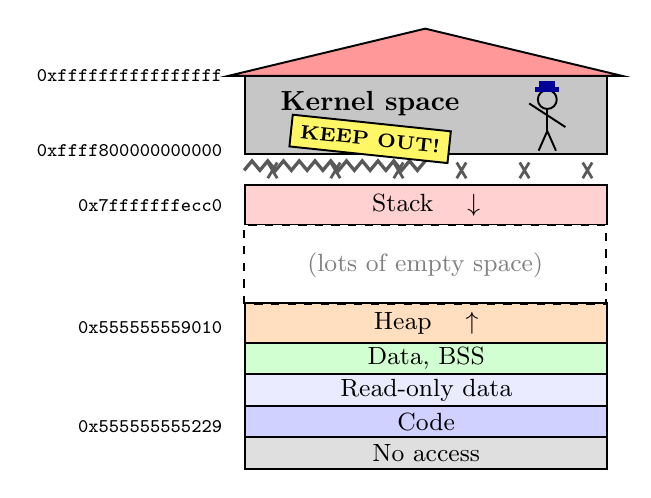
\begin{tikzpicture}[
      floor/.style={draw, minimum width=46mm, anchor=south west, inner sep=0pt, font=\small},
      addr/.style={font=\ttfamily\scriptsize, anchor=east},
      line width=0.7pt,
    ]
    \node[floor, minimum height=4mm, fill=gray!25]   at (0,0)    {No access};
    \node[floor, minimum height=4mm, fill=blue!18]   at (0,0.4)  {Code};
    \node[floor, minimum height=4mm, fill=blue!8]    at (0,0.8)  {Read-only data};
    \node[floor, minimum height=4mm, fill=green!18]  at (0,1.2)  {Data, BSS};
    \node[floor, minimum height=5mm, fill=orange!25] at (0,1.6)  {Heap \quad $\uparrow$};
    \draw[dashed] (0,2.1) rectangle (4.6,3.1);
    \node[font=\small, gray] at (2.3,2.6) {(lots of empty space)};
    \node[floor, minimum height=5mm, fill=red!18]    at (0,3.1)  {Stack \quad $\downarrow$};
    % Barbed wire
    \draw[gray!70!black, line width=1.2pt]
      (0,3.8) \foreach \k in {1,...,23} { -- ++(0.1,{mod(\k,2) ? 0.12 : -0.12}) };
    \foreach \k in {0.3,1.1,1.9,2.7,3.5,4.3}
      \draw[gray!70!black, line width=1pt] (\k,3.7) -- ++(0.12,0.2) (\k+0.12,3.7) -- ++(-0.12,0.2);
    \node[floor, minimum height=10mm, fill=gray!45] at (0,4.0) {};
    \node[font=\bfseries] at (1.6,4.65) {Kernel space};
    \node[draw, fill=yellow!60, font=\scriptsize\bfseries, rotate=-6] at (1.6,4.2) {KEEP OUT!};
    % Guard
    \draw (3.85,4.7) circle (0.12);
    \fill[blue!60!black] (3.7,4.8) rectangle (4.0,4.86);
    \fill[blue!60!black] (3.75,4.86) rectangle (3.95,4.94);
    \draw (3.85,4.58) -- (3.85,4.3);
    \draw (3.85,4.3) -- (3.74,4.05) (3.85,4.3) -- (3.96,4.05);
    \draw (3.85,4.5) -- (3.62,4.65);
    \draw (3.85,4.5) -- (4.08,4.35);
    \filldraw[fill=red!40] (-0.2,5.0) -- (2.3,5.6) -- (4.8,5.0) -- cycle;
    \node[addr] at (-0.15,0.55) {0x555555555229};
    \node[addr] at (-0.15,1.8)  {0x555555559010};
    \node[addr] at (-0.15,3.35) {0x7fffffffecc0};
    \node[addr] at (-0.15,4.05) {0xffff800000000000};
    \node[addr] at (-0.15,5.0)  {0xffffffffffffffff};
  \end{tikzpicture}
  \caption{Memory layout of a 64-bit program (for reference; floor heights not to scale)}
  \label{fig:layout64}
\end{figure}

\section{The Stack: A Pile of Plates, Upside Down}
\label{sec:stack}

\subsection{Meet Functions First}

Before we can talk about the stack, we need to meet \emph{functions}. A function is a piece of code with a name, just like \texttt{main}. We can write our own:

\codefile{code/en/ch04/func.c}{Writing a function of our own}{lst:func}

\inputminted[linenos=false]{text}{code/en/ch04/out/func.txt}

\texttt{int add(int x, int y)} means: this function is called \texttt{add}; it takes two integers, \texttt{x} and \texttt{y} (these are its \emph{parameters}), and when it is done it hands back an integer. \texttt{return sum;} hands back the value of \texttt{sum}. Writing \texttt{add(3, 4)} in \texttt{main} \emph{calls} the function: 3 goes into \texttt{x}, 4 goes into \texttt{y}, the code of \texttt{add} runs, and the 7 it hands back goes into \texttt{c}.

If a function does not need to hand anything back, write its return type as \texttt{void}. If it needs no parameters, write \texttt{void} inside the parentheses too. A function must be written before the place where it is called, so that the compiler knows about it.

\subsection{Function Calls and the Stack}

Variables inside a function, such as \texttt{sum} inside \texttt{add}, are called \emph{local variables}. Where do they live? In the next program, \texttt{main} calls \texttt{first}, \texttt{first} calls \texttt{second}, and \texttt{second} calls \texttt{third}. Each function prints the address of its own local variable:

\codefile{code/en/ch04/stack.c}{Calling one level deeper each time}{lst:stack}

\inputminted[linenos=false]{text}{code/en/ch04/out/stack.txt}

The deeper the call, the smaller the address: each level is \texttt{0x20}, or 32 bytes, below the one before. Every time a function is called, the program marks off a piece of the \emph{stack} for it, called the function's \emph{stack frame}\lazynote{Stack frame}{The piece of the stack used by one function call. It holds the function's local variables and a few other things.}, to hold its local variables. When the function returns, that piece is given back.

The stack is like a pile of plates: each time a function is called, a plate is put on top; when the function returns, the top plate is taken away. The last plate on is the first plate off, and that is exactly how function calls work---\texttt{third} is called last but returns first. There is just one twist: the pile of plates in memory is upside down. It starts at a high address and grows towards lower addresses (Figure~\ref{fig:plates}).

\begin{figure}[htbp]
  \centering
  \begin{tikzpicture}[line width=0.7pt]
    % Ceiling
    \fill[brown!30] (-2.6,0.15) rectangle (2.6,0.45);
    \draw (-2.6,0.15) -- (2.6,0.15);
    \foreach \x in {-2.4,-2.0,...,2.4} \draw[brown!60] (\x,0.45) -- ++(0.25,-0.3);
    % Plates piled upside down
    \foreach \i/\n/\a in {0/main/fdf8, 1/first/fdd8, 2/second/fdb8, 3/third/fd98} {
      \pgfmathsetmacro\y{-0.35-\i*0.62}
      \filldraw[fill=white]  (0,\y) ellipse (1.7 and 0.3);
      \filldraw[fill=cyan!8] (0,\y) ellipse (1.15 and 0.19);
      \node[font=\ttfamily\small] at (0,\y) {\n};
      \node[font=\ttfamily\scriptsize, anchor=west] at (2.0,\y) {0xbfff\a};
    }
    \node[font=\small, anchor=west] at (2.0,0.6) {address};
    % A little person looking up
    \draw (-0.2,-3.35) circle (0.17);
    \draw (-0.2,-3.52) -- (-0.2,-4.05);
    \draw (-0.2,-4.05) -- (-0.38,-4.50) (-0.2,-4.05) -- (-0.02,-4.50);
    \draw (-0.2,-3.70) -- (-0.5,-3.45);
    \draw (-0.2,-3.70) -- (0.1,-3.45);
    \node[red!70!black, font=\Large\bfseries] at (0.45,-3.05) {?!};
    \draw[gray, line width=1pt] (-2.6,-4.50) -- (2.6,-4.50);
    % Note
    \draw[-{Stealth}, thick] (-2.3,-0.4) -- node[left, align=right, font=\small] {one more call,\\one more plate\\underneath} (-2.3,-2.2);
  \end{tikzpicture}
  \caption{The stack is a pile of plates hanging down from the ceiling}
  \label{fig:plates}
\end{figure}

This has two important consequences:
\begin{itemize}
  \item \textbf{Local variables are ``short-stay guests''.} As soon as a function returns, its plate is taken away and its local variables no longer exist. That space is soon taken by the next function call. So never carry the address of a local variable out of its function and use it later.
  \item \textbf{The stack is limited.} On our Linux, a program's stack can be at most 8\,MB (the command \texttt{ulimit -s} shows the limit, in KB). If functions keep calling and calling without end, the pile of plates keeps growing until the stack is used up, and the program crashes. This is called a \emph{stack overflow}\lazynote{Stack overflow}{The stack runs out because calls go too deep or local variables are too big.}. That is where Stack Overflow, the question-and-answer website programmers visit more than any other, got its name.
\end{itemize}

\section{The Heap: Borrowed Memory---Remember to Give It Back}
\label{sec:heap}

The stack is very convenient: memory is handed out automatically when you enter a function and taken back automatically when you leave. But it has two limits: its size is limited, and local variables do not outlive their function. If you do not know in advance how much memory you need (say, to store the scores of everyone in your class, when you only find out how many students there are while the program runs), or if a piece of memory must still be used after a function returns, you need the \emph{heap}.

The heap is a big empty plot of land, and a program can ``borrow'' from it while it runs:
\begin{itemize}
  \item \texttt{malloc(n)} borrows \texttt{n} bytes and hands back the address of that memory. If it cannot borrow them, it hands back \texttt{NULL} (a special address that means ``nowhere'').
  \item \texttt{free(address)} gives borrowed memory back.
\end{itemize}
They are declared in \texttt{stdlib.h}. To really use the borrowed memory we need pointers; Section~\ref{sec:heap-pointer} shows a complete example.

Unlike the stack, memory on the heap is not given back automatically: whatever you borrow, you must return. Forget to \texttt{free} it, and that memory stays taken, and nobody can use it. This is called a \emph{memory leak}\lazynote{Memory leak}{Memory borrowed with \texttt{malloc} but never given back with \texttt{free}; it stays taken and nobody can use it.}. Leaking a little now and then is not a big problem: when a program ends, the operating system takes back all the memory it used. But programs like web browsers and servers run for days on end. If they keep leaking, their memory gets eaten up bit by bit, like a leaky bucket (Figure~\ref{fig:leak}).

\begin{figure}[htbp]
  \centering
  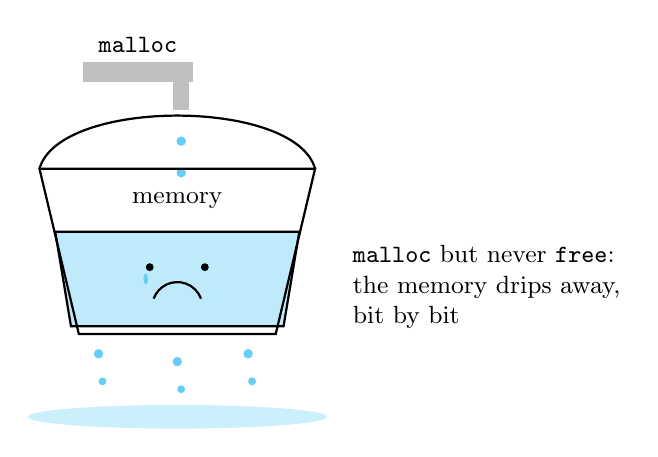
\begin{tikzpicture}[line width=0.8pt]
    % Tap
    \fill[gray!50] (-0.3,3.2) rectangle (1.1,3.45);
    \fill[gray!50] (0.85,3.2) rectangle (1.05,2.85);
    \node[font=\ttfamily\small, anchor=south] at (0.4,3.45) {malloc};
    \foreach \y in {2.45,2.05} \fill[cyan!60] (0.95,\y) circle (0.06);
    % Bucket
    \filldraw[fill=cyan!25] (-0.45,0.1) -- (2.25,0.1) -- (2.45,1.3) -- (-0.65,1.3) -- cycle;
    \draw (-0.85,2.1) -- (2.65,2.1) -- (2.15,0) -- (-0.35,0) -- cycle;
    \draw (-0.85,2.1) .. controls (-0.6,3.0) and (2.4,3.0) .. (2.65,2.1);
    \node[font=\small] at (0.9,1.7) {memory};
    % Crying face
    \fill (0.55,0.85) circle (0.05) (1.25,0.85) circle (0.05);
    \draw (0.6,0.45) arc[start angle=160, end angle=20, radius=0.32];
    \fill[cyan!60] (0.5,0.7) ellipse (0.03 and 0.07);
    % Holes and drops
    \foreach \x/\y in {-0.1/-0.25, 0.9/-0.35, 1.8/-0.25} {
      \fill[cyan!60] (\x,\y) circle (0.06);
      \fill[cyan!60] (\x+0.05,\y-0.35) circle (0.05);
    }
    \fill[cyan!20] (0.9,-1.05) ellipse (1.9 and 0.15);
    \node[font=\small, anchor=west, align=left] at (3.0,0.6)
      {\texttt{malloc} but never \texttt{free}:\\the memory drips away,\\bit by bit};
  \end{tikzpicture}
  \caption{A memory leak}
  \label{fig:leak}
\end{figure}

There are two even worse mistakes: using a piece of memory after giving it back (use after free), and giving the same piece back twice (double free). What happens then is hard to predict. The program may crash on the spot, or it may go wrong in strange ways much later. The example code of Chapter~\ref{chap:c-structure} uses AddressSanitizer to catch this kind of bug, and so does \texttt{make test} in this chapter.

\section{User Space and Kernel Space}
\label{sec:kernel-space}

The operating system's \emph{kernel} has to live in memory too. The kernel runs the whole computer: how memory is shared out, which program runs next, how files are stored, how the keyboard and screen are used---the kernel decides all of it. If any program could change the kernel's data, a buggy program (or a program written by a bad guy) could bring down the whole system. So the place where the kernel lives must be protected.

\subsection{The 32-Bit Split: 3 GB and 1 GB}

On 32-bit Linux, the 4\,GB address space of every program is split into two parts (Figure~\ref{fig:split32}). The lower 3\,GB, from \texttt{0x00000000} to \texttt{0xbfffffff}, is \emph{user space}, where our own program lives. The upper 1\,GB, from \texttt{0xc0000000} to \texttt{0xffffffff}, is \emph{kernel space}, where the kernel's code and data live. Every program has the same kernel living on its top floor.

\begin{figure}[htbp]
  \centering
  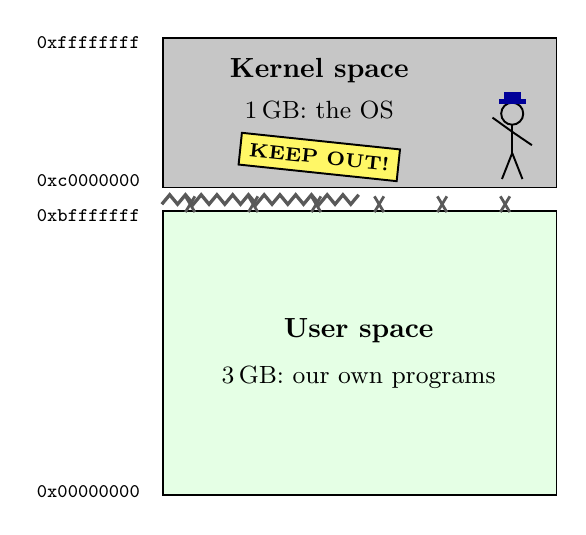
\begin{tikzpicture}[
      floor/.style={draw, minimum width=50mm, anchor=south west, inner sep=0pt},
      addr/.style={font=\ttfamily\scriptsize, anchor=east},
      line width=0.7pt,
    ]
    % User space
    \node[floor, minimum height=36mm, fill=green!10] at (0,0) {};
    \node[font=\bfseries] at (2.5,2.1) {User space};
    \node[font=\small] at (2.5,1.5) {3\,GB: our own programs};
    % Barbed wire
    \draw[gray!70!black, line width=1.2pt]
      (0,3.7) \foreach \k in {1,...,25} { -- ++(0.1,{mod(\k,2) ? 0.12 : -0.12}) };
    \foreach \k in {0.3,1.1,1.9,2.7,3.5,4.3}
      \draw[gray!70!black, line width=1pt] (\k,3.6) -- ++(0.12,0.2) (\k+0.12,3.6) -- ++(-0.12,0.2);
    % Kernel space
    \node[floor, minimum height=19mm, fill=gray!45] at (0,3.9) {};
    \node[font=\bfseries] at (2.0,5.4) {Kernel space};
    \node[font=\small] at (2.0,4.9) {1\,GB: the OS};
    \node[draw, fill=yellow!60, font=\scriptsize\bfseries, rotate=-6] at (2.0,4.3) {KEEP OUT!};
    % Guard
    \draw (4.45,4.85) circle (0.14);
    \fill[blue!60!black] (4.28,4.97) rectangle (4.62,5.04);
    \fill[blue!60!black] (4.34,5.04) rectangle (4.56,5.13);
    \draw (4.45,4.71) -- (4.45,4.35);
    \draw (4.45,4.35) -- (4.32,4.02) (4.45,4.35) -- (4.58,4.02);
    \draw (4.45,4.62) -- (4.2,4.8);
    \draw (4.45,4.62) -- (4.7,4.45);
    % Addresses
    \node[addr] at (-0.15,0.05) {0x00000000};
    \node[addr] at (-0.15,3.55) {0xbfffffff};
    \node[addr] at (-0.15,4.0)  {0xc0000000};
    \node[addr] at (-0.15,5.75) {0xffffffff};
  \end{tikzpicture}
  \caption{The classic split of 32-bit Linux}
  \label{fig:split32}
\end{figure}

This is just what we saw in Figure~\ref{fig:layout}: the stack lives at \texttt{0xbffffdec}, not far below \texttt{0xc0000000}, and above that is kernel space.

\paragraph{On your computer, the stack may live higher up.}
Our computer actually runs 64-bit Linux, and its kernel lives at the top of the 64-bit address space, nowhere near the 4\,GB of a 32-bit program. So on 64-bit Linux a 32-bit program can use all 4\,GB by default, and its stack lives up near addresses like \texttt{0xffff....}, close to the very top. When this book runs 32-bit programs, it makes them use only the lower 3\,GB on purpose, just as on real 32-bit Linux.

\subsection{The 64-Bit Split}

64-bit Linux is split in two in the same way, only with much bigger addresses (Table~\ref{tab:split}). The huge stretch of addresses in the middle cannot be used, precisely because x86-64 processors use only 48-bit addresses (Section~\ref{sec:bits}).

\begin{table}[htbp]
  \centering
  \caption{The address split of x86-64 Linux (48-bit addresses)}
  \label{tab:split}
  \small
  \begin{tabular}{lll}
    \toprule
    Address range & Belongs to & Size \\
    \midrule
    \texttt{0x0000000000000000}--\texttt{0x00007fffffffffff} & user space & 128\,TB \\
    \texttt{0x0000800000000000}--\texttt{0xffff7fffffffffff} & cannot be used & \\
    \texttt{0xffff800000000000}--\texttt{0xffffffffffffffff} & kernel space & 128\,TB \\
    \bottomrule
  \end{tabular}
\end{table}

\subsection{The CPU Guards the Gate}

The protection is done by the CPU's hardware. The CPU has two modes of work: when it runs kernel code it is in \emph{kernel mode}\lazynote{Kernel mode / user mode}{The CPU's two modes of work. Only kernel mode may touch kernel memory and run privileged instructions.}, and when it runs ordinary programs it is in \emph{user mode} (x86 calls them ring 0 and ring 3; RISC-V calls them S-mode and U-mode). Every page of the kernel's memory is marked ``kernel mode only''. Each time the CPU touches memory, it checks: if it is in user mode but wants to touch kernel memory, it refuses at once and tells the kernel to deal with it. The kernel deals with it very simply: it ends the program.

Don't believe it? Try it. As we said earlier, on our 64-bit Linux the kernel is not inside the 4\,GB of a 32-bit program, so this example is built as a 64-bit program (in the \texttt{Makefile}, \texttt{kernel} is built without \texttt{-m32}). It writes a number to an address in 64-bit kernel space. \texttt{0xffffffff81000000} is where the code of the x86-64 Linux kernel usually lives:

\codefile{code/en/ch04/kernel.c}{Writing a number into kernel space (64-bit)}{lst:kernel}

\inputminted[linenos=false]{text}{code/en/ch04/out/kernel.txt}

After printing the first line, the program is stopped at the line \texttt{*p = 42;}, and ``Done!'' is never printed. (What \texttt{*p = 42} means is explained in the next section.) The shell tells us that the program hit a \emph{segmentation fault}\lazynote{Segmentation fault}{The program touched memory it is not allowed to touch, and the OS ended it.}: it touched memory it was not allowed to touch. \texttt{echo \$?} shows that the program's exit status is 139, which is $128 + 11$; 11 is the number of the segmentation fault signal (SIGSEGV).

\begin{figure}[htbp]
  \centering
  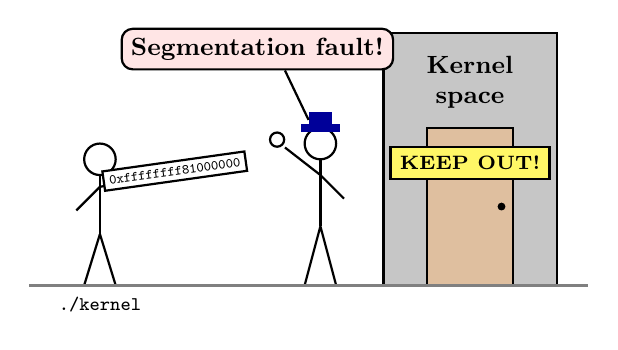
\begin{tikzpicture}[line width=0.8pt]
    % The kernel's gate
    \filldraw[fill=gray!45] (4.2,0) rectangle (6.4,3.2);
    \filldraw[fill=brown!50] (4.75,0) rectangle (5.85,2.0);
    \fill (5.7,1.0) circle (0.05);
    \node[font=\small\bfseries, align=center, inner sep=1pt] at (5.3,2.58) {Kernel\\space};
    \node[draw, fill=yellow!60, font=\scriptsize\bfseries] at (5.3,1.55) {KEEP OUT!};
    % Guard
    \draw (3.4,1.8) circle (0.2);
    \fill[blue!60!black] (3.15,1.95) rectangle (3.65,2.05);
    \fill[blue!60!black] (3.25,2.05) rectangle (3.55,2.2);
    \draw (3.4,1.6) -- (3.4,0.75);
    \draw (3.4,0.75) -- (3.2,0) (3.4,0.75) -- (3.6,0);
    \draw (3.4,1.4) -- (3.7,1.1);
    \draw (3.4,1.4) -- (2.95,1.75);
    \draw (2.85,1.85) circle (0.09);
    % The program, holding a note with the address
    \draw (0.6,1.6) circle (0.2);
    \draw (0.6,1.4) -- (0.6,0.65);
    \draw (0.6,0.65) -- (0.4,0) (0.6,0.65) -- (0.8,0);
    \draw (0.6,1.25) -- (0.3,0.95);
    \draw (0.6,1.25) -- (1.1,1.35);
    \node[draw, fill=white, font=\ttfamily\tiny, rotate=8, inner sep=2pt] at (1.55,1.45) {0xffffffff81000000};
    \node[font=\scriptsize\ttfamily] at (0.6,-0.25) {./kernel};
    % Speech bubble
    \node[draw, rounded corners, fill=red!10, font=\small\bfseries, align=center] (stop) at (2.6,3.0) {Segmentation fault!};
    \draw (stop.south) ++(0.35,0) -- (3.25,2.1);
    \draw[gray, line width=1pt] (-0.3,0) -- (6.8,0);
  \end{tikzpicture}
  \caption{A user program tries to break into kernel space}
  \label{fig:guard}
\end{figure}

So if a user program wants to use the screen or read a file, but may not touch anything of the kernel's, what can it do? The answer: go to the ``counter''. At a bank, you cannot walk into the vault and take money yourself. You hand a form across the counter, and a member of staff fetches it for you. That counter is the \emph{system call}. Remember Section~\ref{sec:runtime}? In the end, \texttt{puts} used the \texttt{write} system call to ask the kernel to put the text on the screen. The CPU has special instructions for this (\texttt{int 0x80} or \texttt{syscall} on x86, \texttt{ecall} on RISC-V). When one of them runs, the CPU switches from user mode to kernel mode and jumps to an entry point the kernel set up in advance. When the kernel has done the job, it switches back to user mode and the program carries on where it left off.

User mode and kernel mode, permission checks on memory, translating virtual addresses into physical addresses---the CPU does all of these in hardware. Anyone who builds their own CPU has to make all of these by hand.

\section{Pointers: A Note with an Address on It}
\label{sec:pointer}

Now we can talk about pointers.

A \emph{pointer}\lazynote{Pointer}{A variable that holds an address. \texttt{p = \&a} makes \texttt{p} point to \texttt{a}; then \texttt{*p} is \texttt{a}.} is also a variable, but what it holds is not an ordinary number---it is an address. It is like a note with the house number of some house written on it. In a 32-bit program an address takes 4 bytes, so a pointer takes 4 bytes; in a 64-bit program a pointer takes 8 bytes (Listing~\ref{lst:bits}).

``Pointer'' is also the name of a breed of hunting dog. When a pointer finds its prey, it freezes, lifts one front paw, and points its nose straight at where the prey is hiding (Figure~\ref{fig:dog}). A pointer in C does the same job: it is not the thing itself, but it tells you where the thing is.

\begin{figure}[htbp]
  \centering
  \begin{tikzpicture}[line width=0.8pt]
    % Tail: held out straight
    \draw[line width=2pt, line cap=round] (-1.05,0.25) -- (-1.95,0.55);
    % Back legs
    \draw[line width=2.4pt, line cap=round] (-0.7,-0.2) -- (-0.85,-1.05);
    \draw[line width=2.4pt, line cap=round] (-0.45,-0.25) -- (-0.4,-1.05);
    % Front legs: one standing, one raised
    \draw[line width=2.4pt, line cap=round] (0.55,-0.25) -- (0.6,-1.05);
    \draw[line width=2.4pt, line cap=round] (0.8,-0.2) -- (1.05,-0.5) -- (0.9,-0.72);
    % Body
    \filldraw[fill=white] (0,0.1) ellipse (1.1 and 0.42);
    \fill[brown!70] (-0.35,0.25) ellipse (0.3 and 0.18);
    \fill[brown!70] (0.3,-0.05) ellipse (0.2 and 0.13);
    % Neck and head
    \filldraw[fill=white] (0.85,0.2) -- (1.15,0.75) -- (1.45,0.65) -- (1.05,0.05) -- cycle;
    \filldraw[fill=white] (1.4,0.75) circle (0.3);
    \filldraw[fill=white] (1.55,0.6) -- (2.05,0.68) -- (2.05,0.85) -- (1.6,0.95) -- cycle;
    \fill (2.05,0.77) circle (0.06);
    \fill (1.5,0.85) circle (0.04);
    \filldraw[fill=brown!70] (1.25,0.95) .. controls (1.05,0.85) and (1.0,0.45) .. (1.2,0.35) .. controls (1.3,0.55) .. (1.38,0.85) -- cycle;
    % Collar and name tag
    \draw[red!70!black, line width=2pt] (1.0,0.62) -- (1.3,0.45);
    \draw (1.15,0.55) -- (0.75,1.0);
    \node[draw, fill=yellow!40, font=\ttfamily\scriptsize, inner sep=2pt, anchor=east] at (0.9,1.1) {p = 0xbffffdf4};
    % Pointing
    \draw[dashed, -{Stealth}, red!70!black] (2.15,0.77) -- (3.85,0.77);
    % Box a
    \filldraw[fill=brown!30] (3.95,0.3) rectangle (5.15,1.25);
    \node[font=\huge\bfseries] at (4.55,0.78) {3};
    \node[draw, fill=yellow!40, font=\ttfamily, rotate=6, inner sep=2pt] at (4.55,0.0) {a};
    \node[font=\ttfamily\scriptsize] at (4.55,-0.45) {lives at 0xbffffdf4};
    \draw[gray, line width=1pt] (-2.1,-1.05) -- (5.5,-1.05);
  \end{tikzpicture}
  \caption{A pointer is like a pointer dog: it is not the prey, but it points to where the prey is}
  \label{fig:dog}
\end{figure}

\codefile{code/en/ch04/pointer.c}{Our first pointer}{lst:pointer}

\inputminted[linenos=false]{text}{code/en/ch04/out/pointer.txt}

There are only three things to write with pointers (Table~\ref{tab:pointer}).

\begin{table}[htbp]
  \begin{lazywide}
  \caption{The three ways of writing pointers}
  \label{tab:pointer}
  \begin{tabular}{L{2.4cm}L{3.4cm}L{6.2cm}}
    \toprule
    Code & Read as & Meaning \\
    \midrule
    \texttt{int *p;} & p is a pointer to int & get a box \texttt{p} that holds the address of an \texttt{int} \\
    \texttt{p = \&a;} & give p the address of a & now \texttt{p} holds the address of \texttt{a}; we say ``\texttt{p} points to \texttt{a}'' \\
    \texttt{*p} & the thing p points to & follow the address in \texttt{p} to its box, and take what is inside \\
    \bottomrule
  \end{tabular}
  \end{lazywide}
\end{table}

So \texttt{*p} is \texttt{a}. Read \texttt{*p}, and you get the value of \texttt{a}, 3. Write 10 into \texttt{*p}, and 10 goes into \texttt{a}'s box, so \texttt{a} becomes 10. \textbf{The most basic use of a pointer is to store data at a given address, or to fetch data from there.}

One thing is easy to mix up: the star \texttt{*} shows up in two places, with two different meanings. In the declaration \texttt{int *p;} it means ``\texttt{p} is a pointer''. In a statement such as \texttt{*p = 10;} it means ``the box that \texttt{p} points to''.

Now look back at \texttt{kernel.c} from the previous section. You can read it now. This line makes \texttt{p} point to an address in kernel space:
\begin{minted}[linenos=false]{c}
int *p = (int *)0xffffffff81000000;
\end{minted}
\texttt{*p = 42;} writes 42 there---and the CPU stops it on the spot. The \texttt{(int *)} in front of the address means ``treat this number as the address of an \texttt{int}''. Just copy it as it is.

\paragraph{Null pointers.}
If a pointer does not point to anything for the moment, set it to \texttt{NULL}. \texttt{NULL} is really just address 0. Remember the ``no access'' floor at the very bottom of Figure~\ref{fig:layout}? Because the area near address 0 cannot be touched, if a program accidentally reads or writes through a \texttt{NULL} pointer, it gets a segmentation fault straight away, instead of quietly messing up data somewhere. The earlier a bug shows up, the easier it is to find.

\section{Solving the Mystery of \texorpdfstring{\NoCaseChange{scanf}}{scanf}: Pointers as Arguments}
\label{sec:swap}

The next program tries to swap the values of two variables:

\codefile{code/en/ch04/swap.c}{Swapping two numbers}{lst:swap}

\inputminted[linenos=false]{text}{code/en/ch04/out/swap.txt}

Why can't \texttt{swap\_wrong} do it? Because when you call a function, it gets \emph{copies} of the values. \texttt{swap\_wrong(a, b)} makes copies of 3 and 4 and puts them into \texttt{x} and \texttt{y} on \texttt{swap\_wrong}'s own plate. It swaps \texttt{x} and \texttt{y}, but \texttt{a} and \texttt{b} on \texttt{main}'s plate are not touched at all (Figure~\ref{fig:swap}, left). When the function returns, its plate is taken away, and the swapped copies go with it.

\texttt{swap}, on the other hand, gets the addresses of \texttt{a} and \texttt{b}. Through \texttt{*x} and \texttt{*y} it follows the addresses and changes the boxes on \texttt{main}'s plate directly, so the swap works (Figure~\ref{fig:swap}, right).

\begin{figure}[htbp]
  \centering
  \begin{tikzpicture}[
      cell/.style={draw, fill=brown!25, minimum width=11mm, minimum height=7mm, font=\ttfamily},
      plate/.style={draw, rounded corners=8pt, fill=cyan!6, minimum width=42mm, minimum height=12mm},
      vname/.style={font=\ttfamily\small, left=1mm},
      line width=0.7pt,
    ]
    \foreach \ox/\who/\xa/\yb/\px/\py/\note in {
        0/swap\_wrong/4/3/3/4/{It swaps the copies;\\\texttt{a} and \texttt{b} don't change},
        5.6/swap/\&a/\&b/4/3/{It follows the addresses\\and changes them: swapped!}} {
      \begin{scope}[xshift=\ox cm]
        \node[plate] (m) at (0,0) {};
        \node[font=\small, above=1mm] at (m.north) {\texttt{main}'s plate};
        \node[cell] (a) at (-0.45,0) {\px};  \node[vname] at (a.west) {a};
        \node[cell] (b) at ( 1.25,0) {\py};  \node[vname] at (b.west) {b};
        \node[plate] (s) at (0,-2.4) {};
        \node[font=\small, below=1mm] at (s.south) {\texttt{\who}'s plate};
        \node[cell] (x) at (-0.45,-2.4) {\xa};  \node[vname] at (x.west) {x};
        \node[cell] (y) at ( 1.25,-2.4) {\yb};  \node[vname] at (y.west) {y};
        \node[font=\small, align=center] at (0,-4.45) {\note};
      \end{scope}
    }
    % Left: the values are copied
    \draw[-{Stealth}, gray, dashed] (-0.45,-0.45) -- node[right, font=\scriptsize] {copy} (-0.45,-1.95);
    \draw[-{Stealth}, gray, dashed] ( 1.25,-0.45) -- node[right, font=\scriptsize] {copy} ( 1.25,-1.95);
    % Right: x and y hold addresses that point to a and b on main's plate
    \fill[yellow!30] (4.6,-2.75) rectangle (5.7,-2.05)  (6.3,-2.75) rectangle (7.4,-2.05);
    \node[cell, fill=yellow!30] at (5.15,-2.4) {\&a};
    \node[cell, fill=yellow!30] at (6.85,-2.4) {\&b};
    \draw[-{Stealth}, red!70!black, thick] (5.15,-2.05) -- (5.15,-0.45);
    \draw[-{Stealth}, red!70!black, thick] (6.85,-2.05) -- (6.85,-0.45);
  \end{tikzpicture}
  \caption{Passing values and passing addresses}
  \label{fig:swap}
\end{figure}

Now we can solve the mystery left over from Section~\ref{sec:scanf}. \texttt{scanf} has to put the number it reads into your variable. If you write \texttt{scanf("\%d", n)}, \texttt{scanf} only gets a copy of the value of \texttt{n}, and it has no way to change the real \texttt{n}. If you write \texttt{scanf("\%d", \&n)}, it gets the address of \texttt{n}, and it can follow the address and put the number there.

If a function wants to change a variable that belongs to its caller, it needs that variable's address. This is the most common use of pointers.

\section{Pointer Plus One: Walking Through Memory}
\label{sec:heap-pointer}

Now we can really put the heap to work. The next program first asks how many students there are, then borrows a block of memory from the system that is just big enough, and stores each student's score in it:

\codefile{code/en/ch04/heap.c}{Storing scores in memory on the heap}{lst:heap}

\inputminted[linenos=false]{text}{code/en/ch04/out/heap.txt}

\begin{itemize}
  \item \texttt{malloc(n * sizeof(int))} borrows a block of memory as big as \texttt{n} \texttt{int}s and puts its address into the pointer \texttt{scores}. After borrowing, check whether you got \texttt{NULL}.
  \item \texttt{scores + i} is the address of box number \texttt{i}, and \texttt{*(scores + i)} is the score in that box. When reading the scores, we hand the address \texttt{scores + i} straight to \texttt{scanf}, with no \texttt{\&}, because it is already an address.
  \item When we are done, \texttt{free(scores)} gives the memory back. Notice that when something goes wrong and the program returns early, it must also \texttt{free} first.
\end{itemize}

Look carefully at the printed addresses: \texttt{0x804d830}, \texttt{0x804d834}, \texttt{0x804d838}. Each one is 4 more than the one before, not 1 more. This is because \texttt{scores} is a pointer to \texttt{int}, and C knows that an \texttt{int} takes 4 bytes. So ``pointer plus one'' means ``move on to the next \texttt{int}'', and the address actually goes up by 4. For a pointer to \texttt{char} (which takes 1 byte), plus one really does add 1 to the address.

\texttt{*(scores + i)} can also be written as \texttt{scores[i]}; the two mean exactly the same thing. The second way of writing it is called an \emph{array}, and we will use it a lot later on.

\section{Writing Data to a Given Address}
\label{sec:mmio}

In the end, a pointer is all about ``writing data to a given address, or reading data from there''. On Linux, a user program may only read and write the addresses the operating system has given it; write to the wrong place and you get a segmentation fault. But what if there is no operating system?

A freshly built CPU has no operating system on it. Among the addresses the CPU can reach there is memory, but there are also all kinds of \emph{devices}: a serial port, a timer, some lights\ldots{} Each device takes up a few addresses. Writing a number to one address might store it in memory; writing to another might send a character out of the serial port, or switch on a light. This is called \emph{memory-mapped I/O}\lazynote{MMIO}{Memory-Mapped I/O: devices take up some addresses, and reading or writing those addresses works the device.}. For example, on the RISC-V virt board emulated by QEMU, the data register of the serial port is at address \texttt{0x10000000}. Write a byte there and a character appears on the screen:
\begin{minted}[linenos=false]{c}
volatile unsigned char *uart = (volatile unsigned char *)0x10000000;

*uart = 'H';
*uart = 'i';
\end{minted}

\texttt{unsigned char} is a type one byte in size, and \texttt{'H'} is the code of the character H. \texttt{volatile} tells the compiler: really do every single read and write, honestly, and don't optimize any of them away (as Chapter~\ref{chap:hello} showed, compilers love to make their own decisions).

This code cannot run directly on Linux---all you would get is a segmentation fault. But on a machine without an operating system, this is the whole secret of ``printing''. \texttt{printf} goes the long way round, through the C standard library, a system call and the operating system's driver, and in the end it does exactly this. The first words a newly built CPU ever says are usually written just like this.

\section{Summary}

\begin{itemize}
  \item Memory is a row of numbered boxes, one byte per box, and the box number is the address. \texttt{\&a} is the address of \texttt{a}; print it with \texttt{\%p}. Both x86 and RISC-V are little-endian.
  \item With $n$-bit addresses you can reach $2^n$ bytes. As memory kept growing, addresses went from 16 bits (64\,KB) to 32 bits (4\,GB), and then to 64 bits. A 32-bit address is 8 hex digits long; all the examples in this chapter use them.
  \item In memory, a program is divided into code, read-only data, data, BSS, heap and stack. Each part has its own read, write and execute permissions, which the CPU checks in hardware. A 64-bit program has the same layout as a 32-bit one, only with longer addresses.
  \item The stack holds the local variables of functions. Each function call adds a stack frame, and returning takes it away. The stack grows from high addresses to low addresses, and its size is limited.
  \item Memory on the heap is borrowed with \texttt{malloc} and given back with \texttt{free}. Forgetting to give it back is a memory leak.
  \item The address space is divided into user space and kernel space. On 32-bit Linux, users get 3\,GB and the kernel gets 1\,GB. If the CPU, in user mode, tries to touch kernel space, it refuses, and the program gets a segmentation fault. User programs ask the kernel to do things for them through system calls.
  \item A pointer is a variable that holds an address: \texttt{p = \&a} makes \texttt{p} point to \texttt{a}, and then \texttt{*p} is \texttt{a}. A function that wants to change its caller's variable needs that variable's address, and that is why \texttt{scanf} needs the \texttt{\&}.
  \item Pointer plus one moves on to the next element; the address goes up by the size of one element.
  \item On a machine without an operating system, writing data to a device's address controls the device.
\end{itemize}

\lazysectionstar{Exercises}

\begin{enumerate}
  \item Add a \texttt{char} variable to Listing~\ref{lst:addr}, and print its address and \texttt{sizeof(char)}.
  \item How many hex digits does a 16-bit address have? How many bytes of memory can a 20-bit address reach?
  \item Build \texttt{layout.c} as both a 32-bit and a 64-bit program (\texttt{gcc -m32 layout.c -o layout32} and \texttt{gcc layout.c -o layout64}) and run each a few times. Which addresses change every time? How do the addresses of the two programs differ? Where does the stack of the 32-bit program live?
  \item Write a function \texttt{void add\_one(int *p)} that adds 1 to the number \texttt{p} points to. Call it from \texttt{main}, and check that the variable really changes.
  \item Change Listing~\ref{lst:heap} so that it also prints the highest score.
  \item Think about it: if a function hands the address of one of its own local variables back to its caller, and the caller then reads through that address, what goes wrong?
  \item Write a program that runs \texttt{int *p = NULL; *p = 1;} and see what happens. Use Figure~\ref{fig:layout} to explain why.
\end{enumerate}
